\documentclass[preprint,12pt]{elsarticle}
%\documentclass{acm_proc_article-sp}
\usepackage[lined,boxed,commentsnumbered, ruled]{algorithm2e}
\usepackage{amssymb,amsmath}
\usepackage{epsfig,graphicx,subfigure}
\usepackage{times}
\usepackage{helvet}
\usepackage{courier}
\usepackage{multirow}
\journal{Information Science}


\begin{document}

\begin{frontmatter}

\title{Finding Contexual Preferrable Products from Online Reviews}
%% use optional labels to link authors explicitly to addresses:
\author{Minyi Cai}
\author{Chen Lin\corref{cor1}}
\ead{chenlin@xmu.edu.cn}
\cortext[cor1]{corresponding author}
\author{Pei Li}
\address{School of Information Science and Engineering, Xiamen University, Xiamen, 361005, China}
\author{Jian Pei}
\address{School of Computing Science, Simon Fraser University, Burnaby, V5A1S6, Canada}


\maketitle
\begin{abstract}

\end{abstract}

\begin{keyword}
%% keywords here, in the form: keyword \sep keyword
%% MSC codes here, in the form: \MSC code \sep code
%% or \MSC[2008] code \sep code (2000 is the default)
\end{keyword}

\end{frontmatter}

%input{}
\section{Introduction}\label{sec:intro}
Product recommender is an indispensible component of modern E-commerce ecosystems. Delivering accurate recommendations benefits both enterprises and consumers. Precise recommendation is built upon fine-tuned modeling of user preferences. As we will soon see in the following example, user preferences are often affected by the ``contexts'', i.e. when, where or with whom the consumptions are made. A context independent recommender will make wrong predictions.

\textbf{Example}: \textit{Bob is looking for a place where he can have his weekday lunch alone. A sandwich combo seems to be a perfect option. The absolute price of item, along with the cleanness and quick service of the restaurant are dominant factors under the context ``weekday lunch for one person''. However, when Bob is preparing for a date with his girlfriend at Christmas' Eve, recommending a fast food restaurant would be inappropriate. Instead, a nice restaurants serving French cuisine and fine wine is more attracting. A reasonably higher price is acceptable, as long as the service and environment is satisfying.}


Context aware recommendation systems (CARS) take  contextual information into account to provide better recommendations. CARS have been successfully applied in a few areas, including travel~\cite{Biancalana2013Approach}, music~\cite{Cai2007MusicSense}, web news~\cite{Wang2015CROWN} and so on. Most state-of-art CARS follow the traditional recommender framework, where context information is either pre-filtered~\cite{Adomavicius2005Incorporating}, post-filtered~\cite{Baltrunas2009Context}, or incorporated in the model~\cite{Palmisano2008Using,Wang2015CROWN,Karatzoglou2010Multiverse}.

Data sparsity is an open problem for recommender systems. It is evern more severe for CARS, since explicit user feedbacks with contexts are often not available. As more and more people share shopping experiences in review sites, recently a few researchers exploit the feasibility of learning context aware user prefernces from online reviews~\cite{Li2010Contextual,Levi2012Finding,Hariri2013Query,Liu2013Combining}. All of them adopt a castcade process, in which they first extract contextual phases and opinions in the reviews, and then implement a contextual aware recommendation system. Online reviews act as complementary ratings, by containing semantic associations among users and products. Moreover, CARS based on text mining have the following advantages. (1) They offer a query driven alternative apart from traditional query independent recommender. Thus they are more friendly for cold-start users. (2) Their results are more intepretable, as the reviews reveal the tastes of consumers. (3) By ensembling heterogeneous relationships (semantic associations in texts and social relationships in collaborative filtering), they are able to generate more diversified recommendations.

Naturally, the performance of recommendation is highly dependent on the performance of context extraction. Online reviews are short textual pieces written in informal natural languages. The extracted contextual ratings are inevitably noisy. This might be the consequence of the ambiguity of natural languages. For example, \textit{``The place is so fun for a date''} is undoubtedly a positive vote for the context ``dating''. But another review (``\textit{I've been going here for years, I won't say how many because that will date myself}'') containing the same word ``date'' is not. It might also be caused by the inconsistency of reviewing and purchasing. For example, the user likes to eat alone in a restaurant, but mentions that it's suitable for a date in the review. Furthermore, it might reflect the fact that opinion mining do not directly lead to preference modeling. For example, opinion mining is a qualitative judgement (positive, neutral and negative), while user preferences are quantified in a numeric manner.

Studies have shown that improper use of contextual information might actually be harmful~\cite{Li2010Contextual}. Unlike previous researches, which attempt to tailor information extraction (IE) techniques for specified context types and domains, this paper focuses on a robust, scalable system which works well with general IE techniques on online reviews. Towards this end, we propose an infrasture which categorizes the extracted contextual phrases and opinions to multiple contexts. It helps to clarify ambigous expressions and to identify the true contexts. Based on utility surplus, we present a probabilistic generative model to learn real-valued contextual aware user preferences and product features from polarized contextual opinions. Three prime issues are addressed. 

Firstly, due to the high volume of online reviews, it is impossible to manually label all context related opinions. We propose a semi-supervised model to learn the hidden contexts from a few roughly labeled instances and a large number of unlabeled instances. We show that the proposed framework outperforms state-of-the-art CARS with or without text mining on real data sets.    

Secondly, we introduce confidence in the recommendation model. Treating reviews as contextual opinions with varing levels of confidences, the system is more false tolerant to inaccurate context extraction and categorization. Our experimental study verifies this point.


Thirdly, we study the mechanism of projecting reviews to coarse grained contexts. Beyond the common multinomial model, which assumes one context for a review instance, and factor model, which assotiates all contexts with an instance, we also present a mediate strategy which links an instance with an appropriate number of contexts. Experimental study demonstrates that this strategy produces the best performances.


The rest of this paper is organized as follows.  We provide a brief discussion on related work in section~\ref{sec:related}. We introduce the overall framework in Sec.~\ref{sec:method}, and its components ( preference quantification model, opinion classification model, and the projection strategies) in section~\ref{sec:util},~\ref{sec:classifier},~\ref{sec:rec} respectfully. The experimental results are described and analyzed in section~\ref{sec:exp}.Finally, we conclude our work in section~\ref{sec:con}.

\section{Related Work}\label{sec:related}
%
CARS based on text mining are genetically related to two areas: contextual aware recommendation systems and online review mining.

\subsection{Contextual Aware Recommendation Systems}

%recsys
Most recommender systems use numeric user ratings to construct a rating matrix, and apply collaborative filtering approaches to recommend items for users with similar tastes~\cite{Bobadilla2013Recommender}. There are two types of collaborative filtering techniques. One is based on retrieving nearest neighbors, performances of which are enhanced by modifying the similarity measurements, such as removing the global effect of nearest neighbors~\cite{Bell2007Scalable}. The other is based on matrix factorization~\cite{Koren2009Matrix} to approximate the observed ratings with hidden user preferences and item features. Probabilistic versions of matrix factorization are also prodominant~\cite{salakhutdinov2008probabilistic}. For binary relevance data, researchers present methodologies that target different object functions, most of which are ranking related measures. For example, BPR~\cite{Rendle2009BPR} maximizes the likelihood of pair-wise rankings, CliMF~\cite{Shi2012CLiMF} directly maximizes the mean reciprocal rank to improve top-k recommendations, ListRank-MF~\cite{Shi2010Listwise} minimizes a loss function that  represents the uncertainty between training lists and output lists.   

%CARS
Constext aware recommender systems (CARS) have attracted both academic and industrial attentions~\cite{Adomavicius2011Context}. The performance of CARS has recently been verified by a live controlled experiment~\cite{Gorgoglione2011Effect}. There are three types of approaches to incorporate contextual information in the recommendation process. The first type is to pre-filter, i.e. select contextualized ratings data and factorize each context specific rating matrix~\cite{Adomavicius2005Incorporating}. The second type is to post-filter, i.e. split the resulting items to different contexts after recommendation~\cite{Baltrunas2009Context}. The third type is to model the context, i.e. as a latent variable in BNN~\cite{Palmisano2008Using}, or as a latent factor in matrix factorization~\cite{Baltrunas2011Context}. or as tensor factorization~\cite{Wang2015CROWN,Karatzoglou2010Multiverse}. Empirical study has shown that which approach is better depends on the application~\cite{Panniello2009Experimental}. The sparsity of rating data is an obstacle for CARS. A typical improvement is to integrate other resources, i.e. demographic information~\cite{Li2011Towards}, sequential patterns~\cite{Hariri2012Context}, or, as we might review in the next subsection, texts in online reviews~\cite{Li2010Contextual,Levi2012Finding,Hariri2013Query,Liu2013Combining}. 



\subsection{Online Review Mining}

Online review  mining has been an active research area. Most existing researches are efforts that summarize reviews and extract certain information, i.e. opinion polarities~\cite{Liu2005Opinion}, user groups according to their interests~\cite{Si2014Users}, aspects of products~\cite{Moghaddam2013FLDA}, and so on. Online review mining often requires a skillful combination of natural language processing (NLP) and machine learning models. An omnipotent model does not exist for every domain. 


Information extracted from online reviews is helpful in recommender systems. For example, identifying product aspects and user opinions is crucial for predicting a user's rating~\cite{Qu2010Bag}, estimating the review quality can "up-weight" or "down-weight" the importance of individual rating while performing collaborative filtering~\cite{Raghavan2012Review}. For CARS, online review mining also assists the recommendation process in POI recommender~\cite{Biancalana2013Approach}, hotel recommender~\cite{Levi2012Finding}, and restaurant recommender\cite{Li2010Contextual}, etc..  


To the best of our knowledge, researches in literature directly utilize the extracted conextual opinions to form the preference data, and conduct models that are essentially similar to CARS without textual input data. For example, a tensor factorization model is presented in ~\cite{Levi2012Finding}, which imitates a user who favors reviews written by people with the same intent, nationality and tasts.  An extended LDA is presented in ~\cite{Hariri2013Query}, which jointly models users, items and contexts. In ~\cite{Li2010Contextual}, the contextural information is integrated into a probabilistic latent relational model, which factorizes ratings to item specific features, as well as a combination of the current context and a user's long term preference. In ~\cite{Liu2013Combining} a simple recommendation model is used to aggregate opinions over each product feature. Altough new features and algorithms are developed, we observe that the majority of former studies achieve accuracies of less than 70$\%$ in contextual opinion extraction. Instead of boosting the precision of contextual opinion mining on certain domains, we attempt to propose a compound recommender, whose recommendation performance will not be deteriorated by the inheritantly imperfectness of contextual opinion extraction.

\section{Methodology Overview}\label{sec:method}

Given a collection of online reviews published by $M$ users on $N$ products,  the context aware recommender aims to rank products according to how they satisfy user needs for each user and a set of contextual conditions, or, alternatively, in the case of cold-start users, for each query $q$ consisting of a set of contextual conditions. We do not limit the form of contextual conditions. They can be any textual phrases in natural languages, i.e. ``\textit{with my girlfriend}'', ``\textit{at Christmas Eve}'', etc. 

CARS based on text mining As mentioned in Sec.~\ref{sec:intro}, we solve this problem by projecting the contextual conditions to some coarse-grained contexts. Fig.~\ref{fig:pgm} depicts how the purchase is made and how a review is written under this assumption.  



In the implied context. We assign a probabilistic score to each restaurant, denoted as $p(c|q)$, the probability of restaurant $c$ being chosen for query $q$. Note that although we require an input query $q$, the methodology can be easily expanded to the usual multi-dimensional $User\times Item \times Context$ settings.

Since the query may match several contexts (i.e. ``with girlfriend, at Christmas Eve.'' can implies ``dating'', ``party'' etc), the probability can be rewritten as  $p(c|q)=\Sigma_x p(c|x)p(x|q)$, where $x$ is a context, the first term is the utility of each restaurant under context $x$, and the second term is the probability of categorizing query $q$ to context $x$.

Consequently, the recommendation framework depicted in Figure~\ref{fig:arch} consists of an off-line learning process and an online recommendation process. The off-line learning process consists of two levels. In the first level, a context classifier  parameterized by $\mathbf{b}$ is trained to predict context label for each unlabeled review $e$. In the second level, the utility quantification model parameterized by $\mathbf{a}$ is learnt for each context from labeled and predicted reviews. The online recommendation uses both $\mathbf{a,b}$ to estimate the final possibility.
\begin{figure}
\centering
\vskip -0.1in
\subfigure[Illustrative probabilistic generative model]{
\includegraphics[width=0.4\textwidth]{PGM.eps}
\label{fig:pgm}}
\subfigure[Castcade solution]
{\includegraphics[width=0.4\textwidth]{architecture.eps}
\label{fig:arch}}
\caption{Framework for context aware recommendation}

\end{figure}


\begin{table}
	\caption{A list of hidden and observed variables and their respective distributions}
	\label{tab:Notations}
	 \begin{tabular}{|cccc|}
	\hline
	\multirow{7}{*}{Hidden variables}& $x$ & purchase context & $x\sim Discrete(x|\sigma_x)$\\ 
	& $u$ & user preference & $u\sim \mathcal{N}(u|0,\sigma_u)$\\ 
	& $v$ & product features & $v\sim \mathcal{N}(v|0,\sigma_v)$\\
	& $a$ & context aware preference & $a\sim \mathcal{N}(a|0,\sigma_a)$\\
	& $r$ & user-product rating & $r_{u,v,x}\sim \mathcal{N}(r|g(u,v,a^x),\sigma_r)$\\
	& $l$ & review context labels & $l\sim Discrete(l|r)$\\
	& $b$ & opinion distribution for each product feature & $b\sim Dirichlet(b|\sigma_b)$\\
	\multirow{2}{*}{Observed variables}& $f$ & a review phrase of product feature & $f\sim q(f|v,\sigma_f)$\\ 
	& o & opinion polarity of product feature & $o\sim Discrete(o|b^l)$\\ \hline
	\end{tabular}
\end{table}


\section{Preference Quantification}\label{sec:util}
%utility
\subsection{Utility Surplus}
Utility is an important property of any commodity. It measures the satisfaction people get by purchasing a commodity. Money, as a special case of commodity, can also be measured by a utility function. If the consumer is willing to pay a certain amount of money, which is the price $c_p$, to purchase a commodity $c$, then the utility surplus $US(c)=UC(c)-UM(c_p)$, which is the commodity utility $UC$ minus the money utility $UM$, will be positive.

Usually, the commodity utility can not be directly counted, but can be inferred from observed consumptions. Moreover, a common assumption is that the commodity utility can be modeled as a linear combination of user preferences over commodity features $UC(c)=\sum_k a_k c_k$, where $a_k$ is the preference to the $k-$th feature $c_k$.

The utility function of money could be more complicated. However, in the coupon recommendation scenario, the consumers are paying a very small portion of money, compared to their income. So according to the law of diminishing marginal utility, a linear function can be adopted to measure the decrease of consumer satisfaction by losing the money, i.e. $UM(c_P)=a_P (-c_P)$. Here $a_P$ can also be interpreted as users preference to price.

Intuitively, the user preferences are context dependent. Therefore, for each coupon $c$, the context aware utility surplus that consumers obtain by paying the coupon price $c_P$, is $US^x(c)$
\begin{equation}\label{equ:us}
  US^x(c)=UC^x(c)-UM^x(c_P)=\sum_k a_k^xc_k + a_P^xc_P
\end{equation}

We make the following manipulation to ensure the score for each coupon coincides with a probability. For a given context $x$, the probability of coupon $c$ being chosen is $p(c|x)$.

\begin{equation}\label{equ:pcx}
  p(c|x)=g(US^x(c))=\frac{1}{1+\exp{-\mathbf{a^x}\mathbf{c}^T}}
\end{equation}
where $\mathbf{a^x}$ is a vector indicating user preferences over commodity features and prices, as well as bias, $\mathbf{a^x}=\{a_0^x,a_1^x,\cdots,a_K^x,a_p^x\}$, and $\mathbf{c}$ is the commodity features and coupon price, as well as a constant feature for bias, $\mathbf{c}=\{1,c_1,\cdots,c_K,c_P\}$. If $US^x(c)>0$, then $p(c|x)>0.5$, which suggests that it is possible to choose the coupon $c$ for context $x$.

\subsection{Utility Learning from Online Reviews}

We should notice that $c_k$ in equation~\ref{equ:us} is in general connected to commodities instead of coupons. We use $c$ to denote both coupon and the corresponding commodity . Given a coupon, its commodity features are known in prior (technical details of extracting commodity features will be discussed in section~\ref{sec:exp}), which leaves only $\mathbf{a^x}$ unknown.  Moreover, user preference $\mathbf{a^x}$ can only be learnt from a set of observations, in our settings, a collection of reviews $E_c$ corresponding to coupon $c$.

Online reviews can be of different formats~\cite{Liu2005Opinion}. We consider the most common type: each review is a brief text message, with the price paid per person $e_P$, and numerical ratings on some general aspects. The consumer may express opinions about the consumption experience in the text message. Intuitively, if a consumer publishes positive comments on a particular context, i.e. ``Nice place for date night'', then in the underlying context $x=\{\textrm{``dating''}\}$, the utility of the commodity is larger than the price, $UC^x(e)>UM^x(e_P)$, as shown in the utility theory. Note that although the characteristics of a commodity are usually fixed, the individual consumption experience may differ due to unpredictable reasons. For example, it is possible that ``restaurant A'' is known for its world-class service, yet some consumers may encounter a rash waiter. So we use $\mathbf{e}$ to denote the specific commodity in review $e$, which is an combination of the commodity features with some mutations observable in the review contents, price $e_P$ paid in the specific experience, and unit feature for bias.

Our basic idea is to use the reviews as positive and negative training samples to learn $\mathbf{a^x}$. We denote the collection of reviews celebrating a good experience in context $x$ as $E^+(x)_c$, and otherwise $E^-(x)_c$. Maximizing the log-likelihood of the training set integrates information over various commodities for a better estimate of $\mathbf{a^x}$. To overcome the shortage of sufficient labeled instances, we train an opinion classifier on the labeled reviews to predict the probability $p(x+|e)$ for any unlabeled review $e$, then we can have more supervision, i.e. a predicted set $L^+(x)_c$ of positive reviews on context $x$ about commodity $c$: $L^+(x)_c=\{<\mathbf{e},l(e)_x>\}$. We have the following loss function, which is a weighted log-likelihood with regularizations.

\begin{equation}\label{equ:lossuu}
\begin{aligned}
    \min_{\mathbf{a^x}}& -\Sigma_{c,e\in L^+(x)_c} \log \frac{1}{1+\exp{-l(e)_x\mathbf{a^x}\mathbf{e}^T}}\\
    &-\Sigma_{c,E^-(x)_c} \log\frac{\exp{-\mathbf{a^x}\mathbf{e}^T}}{1+\exp{-\mathbf{a^x}\mathbf{e}^T}}+\lambda_u\|\mathbf{a^x}\|_2
\end{aligned}
\end{equation}

where $l(e)_x\equiv 1$ for a labeled review by human annotation, and otherwise it is automatically computed by the model introduced in section~\ref{sec:classifier}.

\section{Opinion Classification}\label{sec:classifier}
Suppose we predefine totally $K$ contexts, and we know the sentimental polarity of each given review is positive, (i.e. the reviews all express positive opinions), then the reviews can be grouped into $K\!+\!1$ categories: $\{E^+(x_1),\cdots, E^+(x_{K}), E^+(x_{K+1})\}$, where $E^+(x_1),\cdots, E^+(x_{K})$ are reviews positive about context $x_1,\cdots,x_K$ respectfully, the last category consists of reviews that doesn't belong to any context. The objective of this section is to infer $p(x|\mathbf{f})$ for a contextual factor vector $\mathbf{f}$ in the review $f$, the probability of a review $f$ being a positive opinion on the context. The contextual factor vector $\mathbf{f}$ is in general not consistent with the commodity feature vector in section~\ref{sec:util}. A softmax~\cite{Heckerman1997Models} regression for this multi-class categorization problem is to minimize:
\begin{equation}\label{equ:softmax}
  \min_{\mathbf{b}} -\Sigma_{k,f\in E^+(x_k)}I(l(f)=k)\log \frac{\exp{\mathbf{b^k}\mathbf{f}}}{\Sigma_k \exp{\mathbf{b^k}\mathbf{f}}}
\end{equation}
where $I(l(f)=k)$ is an indicator function that the review is labeled as a positive opinion on context $x^k$ by human annotators. And the context distribution of $\mathbf{f}$ is then computed by $p(l(f)=k|\mathbf{f})=\frac{\exp{\mathbf{b}^k\mathbf{f}^T}}{\Sigma_{k'}\exp{\mathbf{b}^{k'}\mathbf{f}^T}}$

A critical property is that there are hidden structures among online reviews, which can be very useful in predicting contexts. We have the following assumptions.
\begin{enumerate}
  \item All reviews are grouped into commodities, which means that, the prior distribution of contexts in each commodity is the prior context distribution of reviews corresponding to the commodity. In fact, if we randomly sample reviews to annotate, then the context distribution of a commodity in the samples is an approximate estimate of true context distribution on the commodity related reviews. For example, if the commodity has a context distribution $\tilde{PX^c}=\{\textrm{``party:''0.1,``banquet:''0.8,``weekday lunch:''0.1}\}$ in the sample set, then we expect the context ``banquet'' is dominant in the unlabeled reviews.
  \item All reviews are written by the same group of people, which means that, the prior distribution of context and non-context related reviews, denoted as $\tilde{PU}$, are shared among all reviews. For example, if in a random sample, $33\%$ percent of reviews are related to at least one context, then we would expect that about $67\%$ percent of unlabeled reviews are not related to any context.
\end{enumerate}
 Note that $\tilde{PX^c}$ is a $K$-dimensional vector, because a commodity is always related to at least one context, and $\tilde{PU}$ is a $2$-dimensional vector, because a review can be unrelated to any context, so we construct $\tilde{P^c}$ as a $K+1$-dimensional vector.
\begin{equation}\label{equ:prior}
\tilde{P_k^c}=
\left\{
\begin{array}{cc}
\tilde{PU_1} \tilde{PX^c_k}& 1\leq k\leq K\\
\tilde{PU_2} &  k = K
\end{array} \right.
\end{equation}
Following the above assumptions, we devise the KL-divergence between distribution of review samples and the estimated distribution in unlabeled reviews $p^c(l|\mathbf{b})$ based on the parameter $\mathbf{b}$.
\begin{equation}\label{equ:KL}
  D(\tilde{p}\|p(l|\mathbf{b}))\!=\!\Sigma_{c}D_{KL}(\tilde{p^c}\|p^c(l|\mathbf{b}))
\end{equation}
Given a set of labeled reviews $E^+$ on commodities $C^+=\{c\}$, and a large number of unlabeled reviews $EU$, in order to learn the classifier parameters $\mathbf{b}$, we first compute the prior distribution $\tilde{p^c}$ by equation~\ref{equ:prior} from $\tilde{PU}$ and $\tilde{PX}$, and then optimize the following loss function.
\begin{equation}\label{equ:cat}
%\begin{aligned}
  \min_{\mathbf{b}}\!-\frac{1}{E^+}\!\log\!p(E^+|\mathbf{b})\!+\!\lambda_pD(\tilde{p}\|p(l|\mathbf{b}))\!+\!\lambda_c\|\mathbf{b}\!\|_2
%\end{aligned}
\end{equation}
where the first term is to maximize the likelihood for generating the labeled reviews, $\frac{1}{E^+}\log p(E^+|\mathbf{b})=\frac{1}{E^+}\sum_{f\in E^+(k)}\log p(l(f)=k|\mathbf{b})$, for all reviews labeled as the $k-$th context; the second term is to maximize the similarity between context distribution from sampled annotations and unlabeled data; the third term is a rugularizer to avoid over-fitting.

\section{Recommendation Model}\label{sec:rec}
%the overall framework
Given a query $q$, consisting of some contextual factors, the context aware coupon recommender aims to rank all the coupons according to how they satisfy user needs in the implied context. We assign a probabilistic score to each coupon, denoted as $p(c|q)$, the probability of coupon $c$ chosen for query $q$.

Since the query may match several contexts, the probability can be rewritten as  $p(c|q)=\Sigma_x p(c|x)p(x|\mathbf{q})$, where $x$ is a context, $p(c|x)$ is the probability of coupon $c$ selected for the underlying context $x$ in the preference quantification model in section~\ref{sec:util}, and $p(x|\mathbf{q})$ is the probability of contextual factor vector $\mathbf{q}$ matching to context $x$. We can view $q$ as a very short review, which explicitly states that the he/she has a wonderful experience under the contextual factors in $\mathbf{q}$. Thus $p(x|\mathbf{q})$ can be inferred by the multi-class categorization model in section~\ref{sec:classifier}. Therefore, we have the definition of coupon score as:
\begin{align}\label{equ:score}
  p(\mathbf{c}|\mathbf{q})\!=\!\sum_x\frac{1}{1\!+\exp{-\mathbf{a^x}\mathbf{c}^T}}
  \frac{\exp{\mathbf{b^x}\mathbf{q}^T}}{\Sigma_{k}\exp{\mathbf{b^k}\mathbf{q}^T}}
\end{align}

where we should point out the price within $\mathbf{c}$ should be coupon price.

Consequently, the learning process for the recommendation model consists of two levels. In the first level, learn $\mathbf{b}$ from labeled reviews $E^+$, predict $l(e)_x=p(l(e)=x|\mathbf{e})$ for each unlabeled review. In the second level, learn $\mathbf{a}$ for each context, from labeled and predicted reviews. %The learning process is depicted in algorithm~\ref{alg:learning}.

%\begin{algorithm}\label{alg:learning}
%\caption{Learning Process for context aware coupon recommendation}
%\KwIn{A set of labeled reviews $E^+=\{E^+(x_1),\cdots, E^+(x_{K})$, $E^+(x_{K+1})\}$ on commodities sets $C+$, $K$ contexts, a set of unlabeled reviews $EU$, coefficients $\lambda_p,\lambda_c,\lambda_u$, and step size $\alpha$}
%\KwOut{$\mathbf{a},\mathbf{b}$}
%Initialize $\mathbf{a},\mathbf{b}$\;
%Compute $\tilde{P^c}$\;
% \While{not convergent}
%{
%\For{$k=1;k \le K+1;k ++$}
%{
%\For{$f \in E^+$}
%{
%$e[k][f]=\exp\mathbf{b}^k\mathbf{f}^T$\;
%}
%}
%\For{$f \in E^+$}
%{
%$s[f]=\Sigma_{k'}\exp\mathbf{b}^{k'}\mathbf{f}^T$\;
%}
%\For{$k=1;k \le K+1;k ++$}
%{
%$p[k][f]=\frac{e[k][f]}{s[f]}$\;
%$s_k^c=\frac{\tilde{p^c_k}}{\Sigma_{f\in EU_c}p[k][f]}$\;
%$\mathbf{\nabla^k}=-\frac{1}{|E^+|}[\Sigma_{f\in E^+(k)}\mathbf{f}(1-p[k][f])]+2\lambda_c \mathbf{b^k}$\;
% $\mathbf{\nabla^k}-=\lambda_p \Sigma_{c\in C^+}\Sigma_{f\in EU_c}\frac{\mathbf{f}p[k][f]}{s[f]}(\Sigma_{k'}s_{k'}^ce[k'][f]-s_k^cs[f])$\;
% $\mathbf{b^k}=\mathbf{b^k}-\alpha\mathbf{\nabla^k} $\;
% }
%}
%\For{$e\in EU$}
%{
%\For{$x=1;x \le K+1;x ++$}
%{
%$l(e)_x=\frac{\exp{\mathbf{b^x}\mathbf{e}}}{\Sigma_k \exp{\mathbf{b^k}\mathbf{e}}}$\;
%}
%\If{$l(e)_{K+1}\leq l(e)_x$}
%{
%$L+(x)\leftarrow e$\;
%}
%}
%\For{$e\in E^+(x)$}
%{
%$l(e)_x=1$\;
%$L+(x)\leftarrow e$\;
%}
%$E^-(x)=\bigcup E^+(\bar{x})$\;
% \While{not convergent}
%{
%\For{$x=1;x \le K;x ++$}
%{
%\For{$e \in E^+$}
%{
%$p[x][e]=\exp{-l(e)_x\mathbf{a^x}\mathbf{e}^T}$\;
%$\mathbf{\nabla^x}=-\Sigma_c[\Sigma_{e\in L^+(x)_c}\frac{\mathbf{e}l(e)_xp[x][e]}{1+p[x][e]}-\Sigma_{e\in E^-(x)_c}\frac{\mathbf{e}}{1+p[x][e]}]+2\lambda_u\mathbf{a^x}$\;
% $\mathbf{a^x}=\mathbf{a^x}-\alpha\mathbf{\nabla^x} $\;
%}
%}
%}
%return $\mathbf{a,b}$\;
%\end{algorithm}
%
%

 One is essentially a multinomial model, where only one context is 

\section{Experiment}\label{sec:exp}
\subsection{Experimental Setup}
We use two real data sets. One is an online review data sets, which is crawled from Chinese largest review sites dianping.com. We will refer this data set as the dianping data set. We crawl a total number of 2593268 reviews on 15292 restaurants located in Beijing. As shown in figure~\ref{fig:dis}, the review distribution is a truncated power-law distribution. The log probability $logp(k)$ of restaurants with $k$ reviews is linear with $log(k)$. The other data set is a coupon data set, provided by our coauthoring company, which contains 56799 coupons, related to 201 restaurants in the dianping data set.
\begin{figure}
\subfigure[Distribution of reviews]{
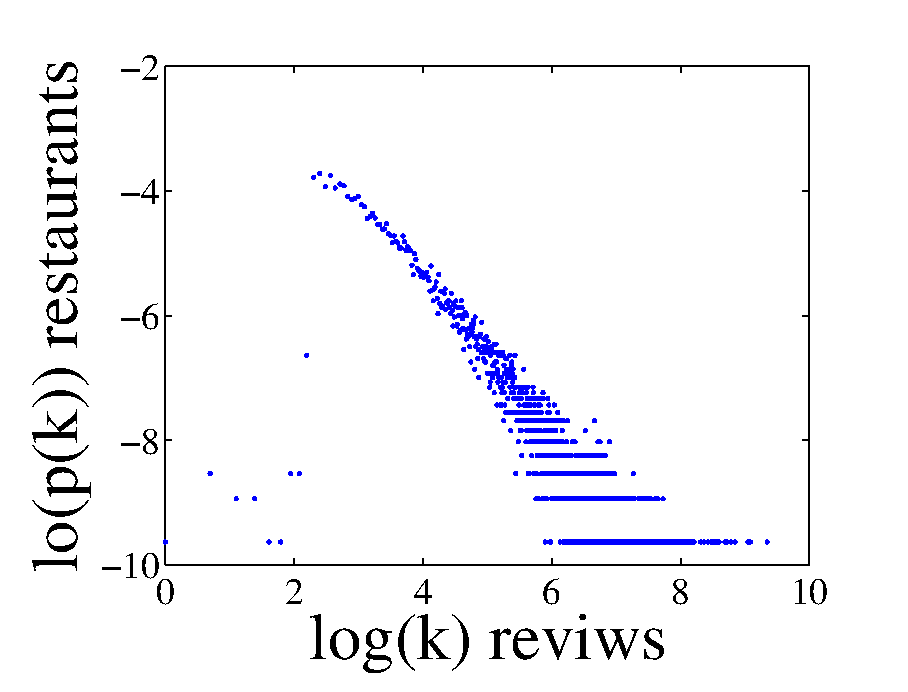
\includegraphics[width=0.22\textwidth]{data.eps}\label{fig:dis}}
\subfigure[Distribution of features]{
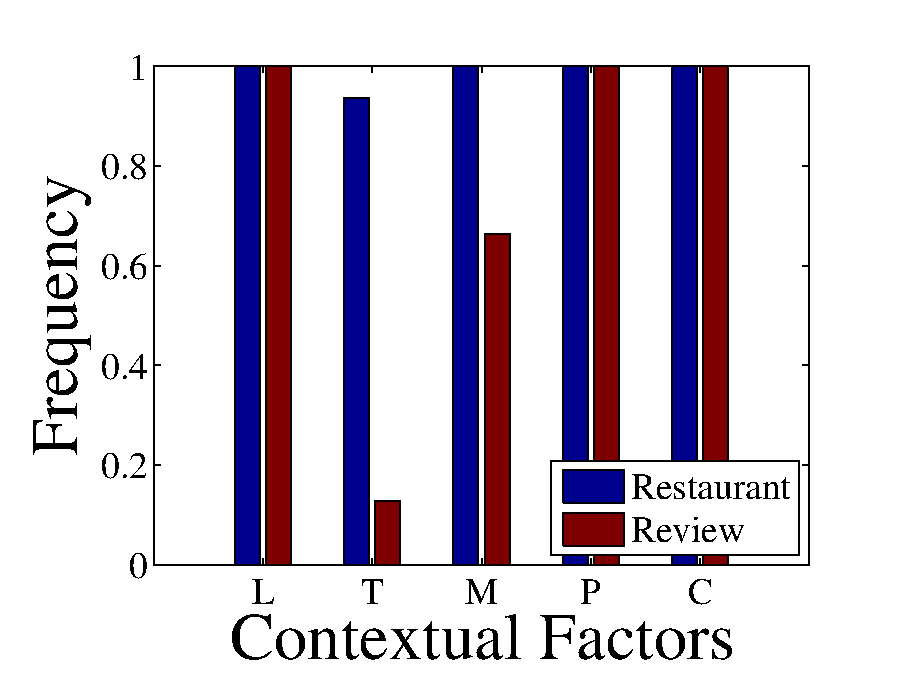
\includegraphics[width=0.22\textwidth]{feature.eps}\label{fig:feat}}
\caption{Statistics of data sets}
\end{figure}

The commodity features are extracted as follows. We first manually build a dictionary containing all the possible aspects of a restaurant, example aspects include ``cuisine'',``food'',``parking'',``service'' and so on. Then we run a sentiment classifier~\cite{Liu2005Opinion} to extract the opinion (positive or negative) of the review on each aspect.  Thus the commodity features are pairs consisting of an aspect and an opinion polarity, e.g. ``food+'' is an extracted feature for the following review phrase ``very good food''. The price demonstrated in a review is usually not the coupon price. In case the price is missing in the review, we use the average price of the restaurant.

The predefined categories for contextual factors used in our experiments include time,location,companion,price and cuisine. We define 5 time factors, including morning, noon, afternoon, night and weekend. Time phrases in a review are matched to one of the 5 time factors. The location factors are collected from dianping, including 43 commercial districts in Beijing. The location factors are identical to all reviews corresponding to the same restaurant. There are 4 types of companion factors(boss, friend, family, couple) and 5 different ranges of number of companions($1,2,3-4,5-10,\geq 10$).The price factors are preprocessed to be 7 categories( $20,20-50,50-80,80-120,120-200,200-500,500-800,\geq 800$). The cuisine factors contain 95 types of cuisines.

All commodity features and contextual factors are binary valued. We count the probability of restaurants and reviews that the contextual factors appear for more than once. As shown in figure~\ref{fig:feat}, cuisine, location and price factors (denoted as ``C'',``L'',and ``P'' in the axis) appear in all restaurants and reviews. A fairy number of people take notes on who they eat with(companion factors denoted as ``M'' in the axis), almost all restaurants have at least one record with companion information. Fewer reviews mention when (time factors denoted as ``T'' in the axis) the experience happens, but the percentage of restaurants with at least one review containing time phrases is much larger.

We define 5 contexts, namely ``Business Banquet'', ``Party'', ``Family Get-together'',`` Dating'' and `` Eat for Leisure''. We pick 27 most popular restaurants and annotate randomly $15\%$ of the reviews (17662 reviews). We observe that the context distribution is unbalanced. Most reviews ($61\%$) are labeled as irrelevant to any context, $19\%$ reviews are labeled to be positive about  ``Party''. We sample $25\%$ of the size of positive instances from the collection of reviews related to each contexts $\bar{x}$, and construct a relatively balanced negative training set  $E^{-}{x}$, with approximately $125\%$ of the size of $E^{+}{x}$. In annotation and opinion categorization, we only deal with reviews with positive opinions. That is, we first filter out reviews with negative opinions. Because there are rare complaining reviews related to a context(could be negative about the overall experience), so for simplicity, we assume we don't have negative opinions in the negative instances. But this can be easily extended.

The step size is set to be $\alpha=1$. The value of $\lambda_p,\lambda_u,\lambda_c$ are decided by cross-validation. For the results below, the values are set to be $\lambda_p=\frac{1}{|EU|},\lambda_u=1,\lambda_c=0.01$

\subsection{Feature Selection Performance}
We first analyze the capability of the preference quantification model and opinion classification model of selecting the most sensitive factors and features to each context. Table~\ref{tab:factor} shows the top features selected with largest $b^x_k$ in time, location, companion, number of companions, price and cuisine factors for each context. Table~\ref{tab:commodity} shows the top 10 commodity features with highest $a^x_k$ in each context. Note that the original features are in Chinese, which are translated to English by Google translator. Although the translation may not represent exactly the same meaning in Chinese, it is enough to demonstrate that the selected features are reasonable for each context.
\begin{table*}[htbp]\label{tab:factor}
\footnotesize
\centering
\caption{The top contextual factors in each group with the largest $b^x_k$}
\begin{tabular}{|c|c|c|c|c|c|}
  \hline
  % after \\: \hline or \cline{col1-col2} \cline{col3-col4} ...
  Context & Banquet & Party & Family & Dating & Leisure \\\hline\hline
  Time & noon & afternoon & noon & weekend & weekend \\\hline
  Loc. & E.40th St. & Houhai& Zoo & Sanlitun & Houhai \\\hline
  Comp. & boss & friend & family & family & family \\\hline
  No. Comp. & 5-10 & 3-4 & 3-4 & 2 & 3-4 \\\hline
  Price & 200-500 & 50-80 & 200-500 & 80-120 & 120-200 \\\hline
  Cuisine & roast duck & hotpot &  Russian & ryori & fastfood \\\hline
\end{tabular}
\end{table*}

\begin{table*}[htbp]\label{tab:commodity}
\footnotesize
\centering
\caption{Top commodity features in each context with the largest $a^x_k$}
\begin{tabular}{|c|c|c|c|c|c|}
  \hline
  % after \\: \hline or \cline{col1-col2} \cline{col3-col4} ...
  Context & Banquet & Party & Family & Dating & Leisure \\\hline\hline
   \#1 & dish+ & texture + & texture+ & environment+ & environment+ \\\hline
   \#2 & cuisine+ & course+& course+ & texture+ & service+ \\\hline
   \#3 & private room+ & waiter+& food container+ & waiter+ &texture+  \\\hline
   \#4 & design+ & environment+ & course- & service+ & design+ \\\hline
   \#5  & menu+ & service+ & texture- & course+ & dish+ \\\hline
   \#6 & dish- & sofa+& design+ & dish+ & course+ \\\hline
   \#7 & course+ & quantity+ &  menu+ & attitude+ & location+ \\\hline
   \#8 & atmosphere+ & food container+ & food container- & quantity+ & atmosphere+ \\\hline
   \#9  & appearance+ & design+ & appearance+ & deal+ & seat+ \\\hline
   \#10 & service+ & dish+ & quantity- & ingredients+ & quantity- \\\hline
\end{tabular}
\end{table*}
We also have some interesting discoveries from table~\ref{tab:factor} and table~\ref{tab:commodity}. (1)People tend to pay more for business banquet and less for a party. (2)People are more tolerant to food and atmosphere when they are getting together with family members, i.e. both positive and negative opinions on food container and course appear, nonetheless, they keep records on them. On the contrary, people are cautious when they are dating with someone, i.e. all features are positive opinions.
\subsection{Semi-supervision Performance}
We next analyze how the semi supervised mechanism works for predicting a similar context distribution in the unlabeled review set as the prior knowledge. Figure~\ref{fig:KL} shows the KL-divergence of the predicted context distribution and the prior distribution from the annotated reviews of sample size $5\%,10\%,15\%$ respectfully. We can see that the KL-divergence is quite small, and is decreasing as the sample size increases.
\begin{figure}
\centering
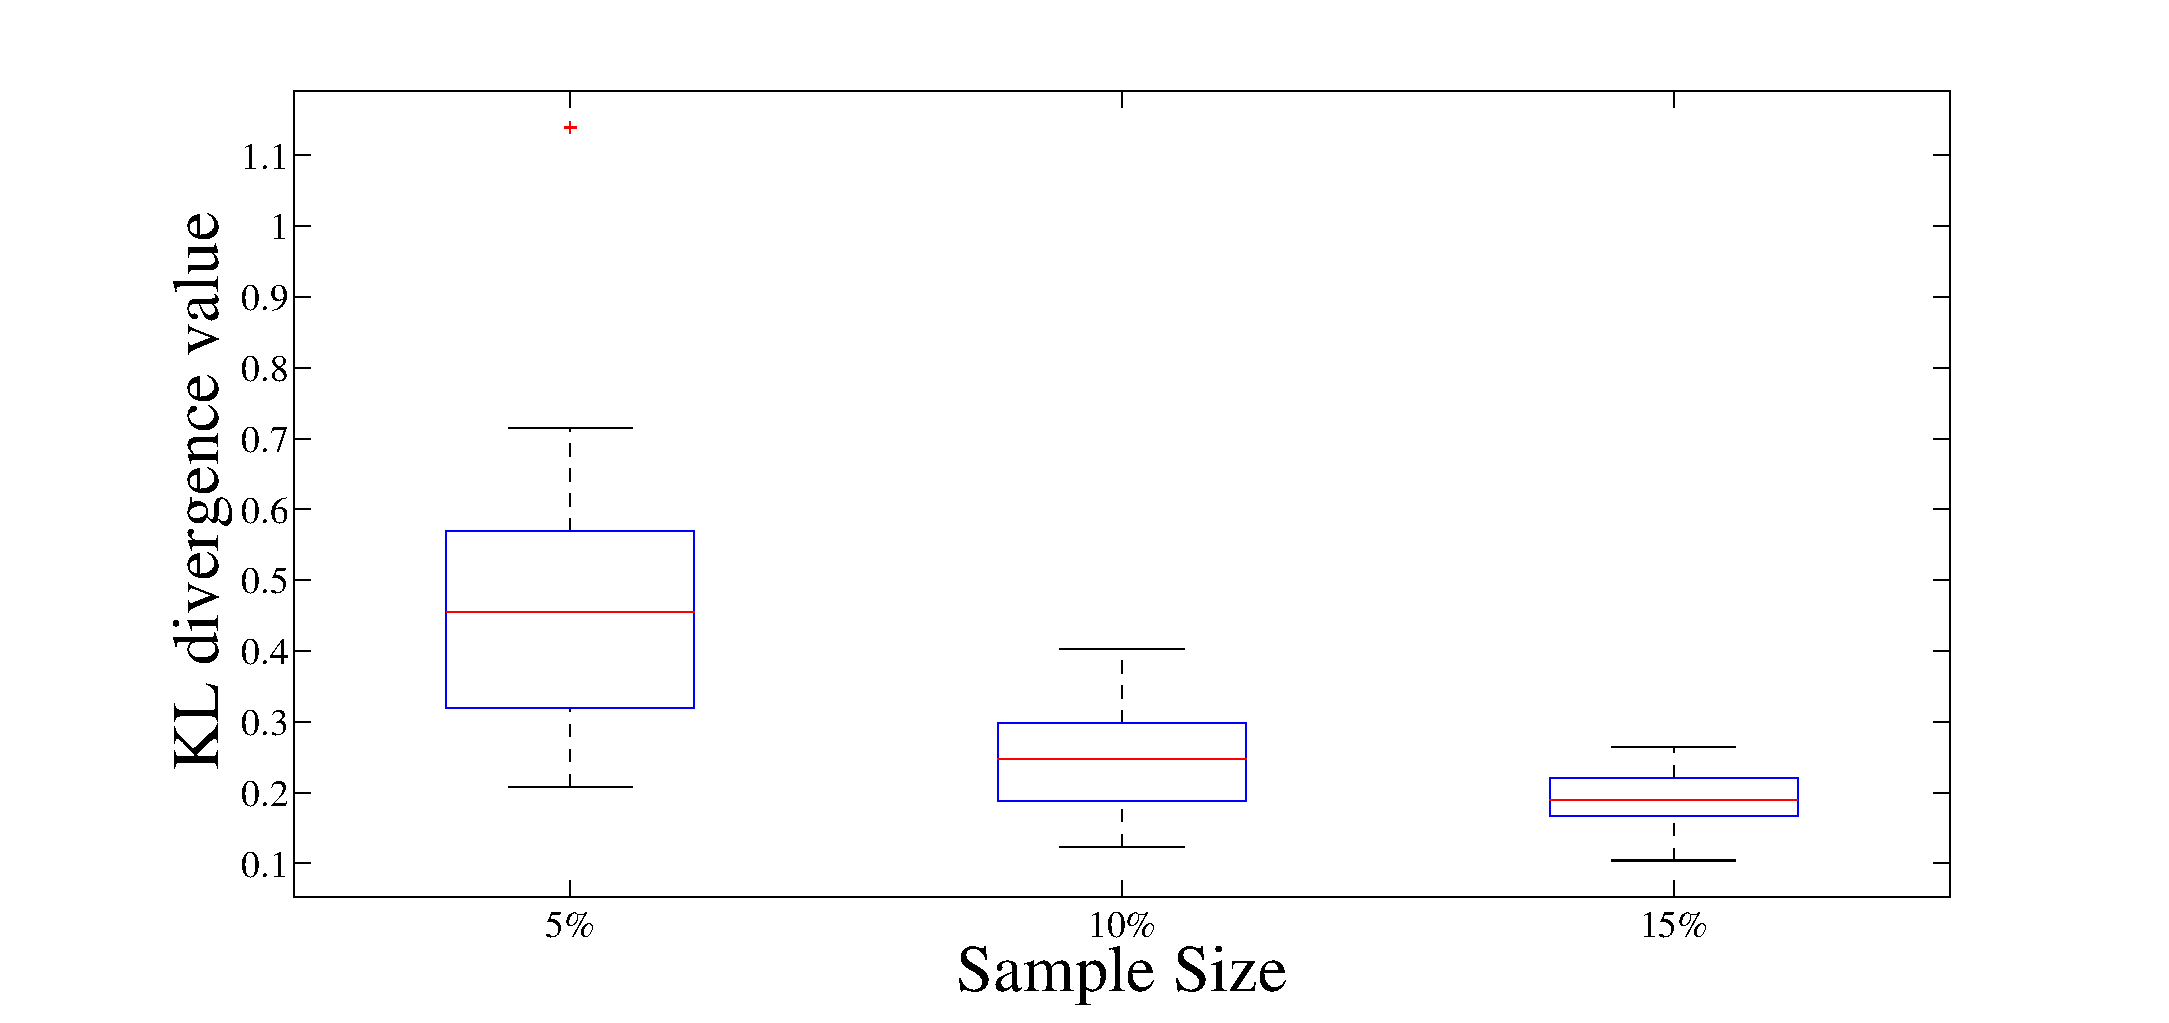
\includegraphics[width=0.4\textwidth]{KL.eps}\label{fig:KL}
\caption{$D_{KL}$ with different sample sizes}
\end{figure}

\subsection{Comparative Study on Context-aware Utility Ranking}
We compare the list of restaurants based on Preference Quantification Model (PQM), with normal price, to the ground truth collected from dianping. There are 6 labels in dianping, the first 4 are equivalent to the contexts we defined, we merge the labels ``eat casually'' and ``eat for leisure'' as the context ``leisure''. The precision in the top ranked restaurants is very high, $P@10,P@30,P@50$ are all equal to 1.

One problem with the ground truth is that, the ground truth is annotated by restaurants holders. Since the restaurants want to expand their target audiences, they tend to assign many labels. To further verify the performance of our context-aware utility ranking, we select top 30 restaurants by PQM, and compute the Jaccard distance between two contexts. We also compare PQM to 4 other ranking machines, the first is the default intelligent ranker in Dianping (DD), the second is order by the number of users(NU), the third is order by the number of reviews(NE), and the fourth is order by the average rating(AR).
\begin{figure}[!hbp]
\centering
\subfigure[DD]{
\includegraphics[width=0.13\textwidth]{CoDianping.eps}\label{fig:dianping}
}
\hspace{0pt}
\vspace{0pt}
\subfigure[NU]{
\includegraphics[width=0.13\textwidth]{CoUser.eps}\label{fig:user}
}
\hspace{0pt}
\vspace{0pt}
\subfigure[NE]{
\includegraphics[width=0.13\textwidth]{CoReview.eps}\label{fig:revew}
}
\hspace{0pt}
\vspace{0pt}
\subfigure[AR]{
\includegraphics[width=0.13\textwidth]{CoRanking.eps}\label{fig:ranking}
}
\hspace{0pt}
\vspace{0pt}
\subfigure[PQM]{
\includegraphics[width=0.13\textwidth]{CoOurs.eps}\label{fig:ours}
}
\caption{Jaccard distance between top 30 restaurants for two different contexts by a ranking mechanism}
\end{figure}

As shown in figure~\ref{fig:dianping}to figure~\ref{fig:ranking}, the Jaccard distance between two sets of top 30 results produced by NU,NE and AR under different contexts are close to 1, which means that the three rankers are not sensitive to context. DD provides more distinguishable results. As shown in figure~\ref{fig:ours}, the Jaccard distances are almost all 0 by PQM, which means that the top 30 results generated by PQM are highly dissimilar in different contexts, with zero overlaps.

\subsection{Visualization of Context-aware Landmarks}
We visualize the performance of context-aware utility ranking. We pick the top 1000 restaurants computed by PQM in each context. The density of restaurant distribution is drawn at a map of Beijing county. As shown in figure~\ref{fig:lm1} to figure~\ref{fig:lm5}, we have the following observations: (1) the best place for business banquet is right in the city center of Beijing; (2) best places for party are more scattered settled; (3) family can get together at any place, but the famous place of interest Xizhimen is the best choice; (4)dating and leisure eating can also take place at anywhere, but the most popular choice is quite different with that people will make for uniting with family members. The most popular choice Sunlitun is a place full of bars. The visualization accord with our common sense.
\begin{figure}
\centering
\subfigure[Business]{
\includegraphics[width=0.13\textwidth]{1.eps}\label{fig:lm1}
}
\subfigure[Party]{
\includegraphics[width=0.13\textwidth]{2.eps}\label{fig:lm2}
}
\subfigure[Family]{
\includegraphics[width=0.13\textwidth]{3.eps}\label{fig:lm3}
}
\subfigure[Dating]{
\includegraphics[width=0.13\textwidth]{4.eps}\label{fig:lm4}
}
\subfigure[Leisure]{
\includegraphics[width=0.13\textwidth]{5.eps}\label{fig:lm5}
}
\caption{Visualization on top 1000 restaurants for each contexts at the map}
\end{figure}
\subsection{Recommendation Performance}
Finally, we analyze the performance of context aware coupon recommendations. We simulate a topic set of 30 queries. Each query has at least one contextual factors, and several freely expressed keywords. We then parse the contextual factors, match the free expressed keywords to commodity features if possible. %Sample queries are listed in table~\ref{tab:query}
%
%\begin{table*}\label{tab:query}
%\small
%\centering
%\caption{Sample queries containing contextual factors}
%\begin{tabular}{|c|c|c|}
%  \hline
%  % after \\: \hline or \cline{col1-col2} \cline{col3-col4} ...
% ID&Original Query&Parsed Query\\\hline
% Q1&have dinner with three friends
%&Time=dinner,Companion= friends, Number of Companions=2-4\\\hline
%Q7&good Sichuan Cuisine suitable for family party
%&Cuisine=Sichuan CuisineìCompanion=family \\\hline
%Q12&good music,date with girlfriend
%&Feature=music+, Companion=girlfriend\\\hline
%Q25&good food near Zhongguancun in Haidian District
%&Location=Zhongguancun in Haidian District,Feature=food+\\\hline
%Q29&price around 100 yuan,have a party with a few friends
%&price=80-120,Companion=friend,Number of Companions=2-4\\\hline
%  \hline
%\end{tabular}
%\end{table*}

We conduct user study on the topic set. We ask 7 undergraduate students, who have no knowledge about which recommender produce which result, to individually rate the top 10 results from the context-aware coupon recommender (CACR) and several other comparative recommenders. The ratings are in range of $[1,5]$, where 1 stands for not interested at all, and 5 stands for highly preferable. We also ask the judges to read the reviews related to each coupon, and decide if the recommendation can be interpreted by the reviews. Score 1 if it can not be explained at all, and 5 if it is completely interpretable from the reviews. We further ask the judges to grade the whole list of coupons based on divergence. Grade 1 if all the coupons are with the same taste, and 5 if there are highly divergent options. The comparative recommenders include: (1) a naive ranker based on price; (2) a naive ranker based on date; (3)a search based ranker Terrier~\cite{Ounis2006Terrier}, which uses the original query as input, and ranks each coupon profile (aggregation of reviews) by BM25.

\begin{table}\label{tab:us}
\centering
\footnotesize
\caption{User Study on Coupon Recommendation}
\begin{tabular}{|c|c|c|c|}
  \hline
  % after \\: \hline or \cline{col1-col2} \cline{col3-col4} ...
  Performance & Rating & Divergence & Interpretability \\\hline\hline
  Price & 3.47 & 2.86 & 1.71 \\
  Date & 3.47 & $\mathbf{4.14}$ & 1.57 \\
  Terrier & 2.91 & $2.57$ & 2.84 \\
  CACR & $\mathbf{4.03}^{++}$ & 3.28 & $\mathbf{4.16}^{++}$ \\
  \hline
\end{tabular}
\end{table}

As shown in table~\ref{tab:us}, CACR performs best in terms of average rating and interpretability, which verifies the effectiveness and context awareness of the recommendation model. The improvements are significant, as $++$ indicates the p-value between the CACR result with the second best result is less than $1\%$. The naive rankers based on price and date perform poorly because they don't personalize recommendations based on the implied context. Their results are not explainable. Ranking by price tends to result in coupons with similar style, i.e. cheap fast foods. A general purpose search engine doesn't perform well, because it is not modified to contextual queries, thus it can not generate truly relevant results.


\section{Conclusion}~\label{sec:con}

\begin{thebibliography}{10}

\bibitem{Adomavicius2005Incorporating}
Gediminas Adomavicius, Ramesh Sankaranarayanan, Shahana Sen, and Alexander
  Tuzhilin.
\newblock Incorporating contextual information in recommender systems using a
  multidimensional approach.
\newblock {\em ACM Trans. Inf. Syst.}, 23(1):103--145, January 2005.

\bibitem{Adomavicius2011Context}
Gediminas Adomavicius and Alexander Tuzhilin.
\newblock Context-aware recommender systems.
\newblock In {\em Recommender systems handbook}, pages 217--253. Springer,
  2011.

\bibitem{Baltrunas2011Context}
Linas Baltrunas, Bernd Ludwig, Stefan Peer, and Francesco Ricci.
\newblock Context-aware places of interest recommendations for mobile users.
\newblock In {\em Design, User Experience, and Usability. Theory, Methods,
  Tools and Practice}, pages 531--540. Springer, 2011.

\bibitem{Baltrunas2009Context}
Linas Baltrunas and Francesco Ricci.
\newblock Context-based splitting of item ratings in collaborative filtering.
\newblock In {\em Proceedings of the Third ACM Conference on Recommender
  Systems}, RecSys '09, pages 245--248, New York, NY, USA, 2009. ACM.

\bibitem{Bell2007Scalable}
R.M. Bell and Y.~Koren.
\newblock Scalable collaborative filtering with jointly derived neighborhood
  interpolation weights.
\newblock In {\em Data Mining, 2007. ICDM 2007. Seventh IEEE International
  Conference on}, pages 43--52. Ieee, 2007.

\bibitem{Biancalana2013Approach}
Claudio Biancalana, Fabio Gasparetti, Alessandro Micarelli, and Giuseppe
  Sansonetti.
\newblock An approach to social recommendation for context-aware mobile
  services.
\newblock {\em ACM Trans. Intell. Syst. Technol.}, 4(1):10:1--10:31, February
  2013.

\bibitem{Bobadilla2013Recommender}
J.~Bobadilla, F.~Ortega, A.~Hernando, and A.~Gutiérrez.
\newblock Recommender systems survey.
\newblock {\em Knowledge-Based Systems}, 46(0):109 -- 132, 2013.

\bibitem{Cai2007MusicSense}
Rui Cai, Chao Zhang, Chong Wang, Lei Zhang, and Wei-Ying Ma.
\newblock Musicsense: Contextual music recommendation using emotional
  allocation modeling.
\newblock In {\em Proceedings of the 15th International Conference on
  Multimedia}, MULTIMEDIA '07, pages 553--556, New York, NY, USA, 2007. ACM.

\bibitem{Gorgoglione2011Effect}
Michele Gorgoglione, Umberto Panniello, and Alexander Tuzhilin.
\newblock The effect of context-aware recommendations on customer purchasing
  behavior and trust.
\newblock In {\em Proceedings of the Fifth ACM Conference on Recommender
  Systems}, RecSys '11, pages 85--92, New York, NY, USA, 2011. ACM.

\bibitem{Hariri2012Context}
Negar Hariri, Bamshad Mobasher, and Robin Burke.
\newblock Context-aware music recommendation based on latenttopic sequential
  patterns.
\newblock In {\em Proceedings of the Sixth ACM Conference on Recommender
  Systems}, RecSys '12, pages 131--138, New York, NY, USA, 2012. ACM.

\bibitem{Hariri2013Query}
Negar Hariri, Bamshad Mobasher, and Robin Burke.
\newblock Query-driven context aware recommendation.
\newblock In {\em Proceedings of the 7th ACM Conference on Recommender
  Systems}, RecSys '13, pages 9--16, New York, NY, USA, 2013. ACM.

\bibitem{Heckerman1997Models}
David Heckerman and Christopher Meek.
\newblock Models and selection criteria for regression and classification.
\newblock In {\em Proceedings of the Thirteenth Conference on Uncertainty in
  Artificial Intelligence}, UAI'97, pages 223--228, San Francisco, CA, USA,
  1997. Morgan Kaufmann Publishers Inc.

\bibitem{Karatzoglou2010Multiverse}
Alexandros Karatzoglou, Xavier Amatriain, Linas Baltrunas, and Nuria Oliver.
\newblock Multiverse recommendation: N-dimensional tensor factorization for
  context-aware collaborative filtering.
\newblock In {\em Proceedings of the Fourth ACM Conference on Recommender
  Systems}, RecSys '10, pages 79--86, New York, NY, USA, 2010. ACM.

\bibitem{Koren2009Matrix}
Y.~Koren, R.~Bell, and C.~Volinsky.
\newblock Matrix factorization techniques for recommender systems.
\newblock {\em Computer}, 42(8):30--37, 2009.

\bibitem{Levi2012Finding}
Asher Levi, Osnat Mokryn, Christophe Diot, and Nina Taft.
\newblock Finding a needle in a haystack of reviews: Cold start context-based
  hotel recommender system.
\newblock In {\em Proceedings of the Sixth ACM Conference on Recommender
  Systems}, RecSys '12, pages 115--122, New York, NY, USA, 2012. ACM.

\bibitem{Li2011Towards}
Beibei Li, Anindya Ghose, and Panagiotis~G. Ipeirotis.
\newblock Towards a theory model for product search.
\newblock In {\em Proceedings of the 20th international conference on world
  wide web}, pages 327--336, 2011.

\bibitem{Li2010Contextual}
Yize Li, Jiazhong Nie, Yi~Zhang, Bingqing Wang, Baoshi Yan, and Fuliang Weng.
\newblock Contextual recommendation based on text mining.
\newblock In {\em Proceedings of the 23rd International Conference on
  Computational Linguistics: Posters}, COLING '10, pages 692--700, Stroudsburg,
  PA, USA, 2010. Association for Computational Linguistics.

\bibitem{Liu2005Opinion}
Bing Liu, Minqing Hu, and Junsheng Cheng.
\newblock Opinion observer: Analyzing and comparing opinions on the web.
\newblock In {\em Proceedings of the 14th International Conference on World
  Wide Web}, WWW '05, pages 342--351, New York, NY, USA, 2005. ACM.

\bibitem{Liu2013Combining}
Hongyan Liu, Jun He, Tingting Wang, Wenting Song, and Xiaoyang Du.
\newblock Combining user preferences and user opinions for accurate
  recommendation.
\newblock {\em Electronic Commerce Research and Applications}, 12(1):14 -- 23,
  2013.

\bibitem{Moghaddam2013FLDA}
Samaneh Moghaddam and Martin Ester.
\newblock {The FLDA model for aspect-based opinion mining: addressing the cold
  start problem}.
\newblock In {\em Proceedings of the 22nd international conference on World
  Wide Web}, pages 909--918. International World Wide Web Conferences Steering
  Committee, May 2013.

\bibitem{Ounis2006Terrier}
I.~Ounis, G.~Amati, V.~Plachouras, B.~He, C.~Macdonald, and C.~Lioma.
\newblock {Terrier: A High Performance and Scalable Information Retrieval
  Platform}.
\newblock In {\em Proceedings of ACM SIGIR'06 Workshop on Open Source
  Information Retrieval (OSIR 2006)}, 2006.

\bibitem{Palmisano2008Using}
C.~Palmisano, A~Tuzhilin, and M.~Gorgoglione.
\newblock Using context to improve predictive modeling of customers in
  personalization applications.
\newblock {\em Knowledge and Data Engineering, IEEE Transactions on},
  20(11):1535--1549, Nov 2008.

\bibitem{Panniello2009Experimental}
Umberto Panniello, Alexander Tuzhilin, Michele Gorgoglione, Cosimo Palmisano,
  and Anto Pedone.
\newblock Experimental comparison of pre- vs. post-filtering approaches in
  context-aware recommender systems.
\newblock In {\em Proceedings of the Third ACM Conference on Recommender
  Systems}, RecSys '09, pages 265--268, New York, NY, USA, 2009. ACM.

\bibitem{Qu2010Bag}
Lizhen Qu, Georgiana Ifrim, and Gerhard Weikum.
\newblock The bag-of-opinions method for review rating prediction from sparse
  text patterns.
\newblock In {\em Proceedings of the 23rd International Conference on
  Computational Linguistics}, COLING '10, pages 913--921, Stroudsburg, PA, USA,
  2010. Association for Computational Linguistics.

\bibitem{Raghavan2012Review}
Sindhu Raghavan, Suriya Gunasekar, and Joydeep Ghosh.
\newblock Review quality aware collaborative filtering.
\newblock In {\em Proceedings of the Sixth ACM Conference on Recommender
  Systems}, RecSys '12, pages 123--130, New York, NY, USA, 2012. ACM.

\bibitem{Rendle2009BPR}
Steffen Rendle, Christoph Freudenthaler, Zeno Gantner, and Lars Schmidt-Thieme.
\newblock Bpr: Bayesian personalized ranking from implicit feedback.
\newblock In {\em Proceedings of the Twenty-Fifth Conference on Uncertainty in
  Artificial Intelligence}, UAI '09, pages 452--461, Arlington, Virginia,
  United States, 2009. AUAI Press.

\bibitem{salakhutdinov2008probabilistic}
R.~Salakhutdinov and A.~Mnih.
\newblock Probabilistic matrix factorization.
\newblock {\em Advances in neural information processing systems},
  20:1257--1264, 2008.

\bibitem{Shi2012CLiMF}
Yue Shi, Alexandros Karatzoglou, Linas Baltrunas, Martha Larson, Nuria Oliver,
  and Alan Hanjalic.
\newblock Climf: Learning to maximize reciprocal rank with collaborative
  less-is-more filtering.
\newblock In {\em Proceedings of the Sixth ACM Conference on Recommender
  Systems}, RecSys '12, pages 139--146, New York, NY, USA, 2012. ACM.

\bibitem{Shi2010Listwise}
Yue Shi, Martha Larson, and Alan Hanjalic.
\newblock List-wise learning to rank with matrix factorization for
  collaborative filtering.
\newblock In {\em Proceedings of the fourth ACM conference on Recommender
  systems}, RecSys '10, pages 269--272, New York, NY, USA, 2010. ACM.

\bibitem{Si2014Users}
Jianfeng Si, Qing Li, Tieyun Qian, and Xiaotie Deng.
\newblock Users’ interest grouping from online reviews based on topic
  frequency and order.
\newblock {\em World Wide Web}, 17(6):1321–1342, 2014.

\bibitem{Wang2015CROWN}
S.~Wang, B.~Zou, C.~Li, K.~Zhao, Q.~Liu, and H.~Chen.
\newblock Crown: A context-aware recommender for web news.
\newblock In {\em 2015 IEEE 31st International Conference on Data Engineering},
  pages 1420--1423, April 2015.

\end{thebibliography}

\end{document}